% % -----------------------------------------------------------------------------
\section{Overview of SBOL}
% % -----------------------------------------------------------------------------

\Rtodo{This section needs review by someone }

Synthetic biology designs can be described using:
\begin{itemize}
\item Structural terms, e.g., a set of annotated sequences or information about chemical makeup.
\item Functional terms, e.g., the way that components might interact with each other and the overall behavior.
\end{itemize}
In broad strokes, SBOL 1.1 focuses on physical, structural information, whereas SBOL 2.0 includes functional aspects. The physical information about a designed genetic circuit includes the order of its constituents and their descriptions. The exact locations of these constituents and their sequences allow genetic circuits to be defined unambiguously, and reused in other designs. SBOL 2.0 extends SBOL 1.1 in several ways: it extends physical descriptions to include entities beyond DNA sequences, and it allows for functional descriptions of the design. 

As an example, consider the design of an expression cassette, such as found in the plasmid pUC18 \cite{L08752.1}, a device that is designed to detect successful versus unsuccessful molecular cloning. As an overall system, the device is designed to grow either blue-colored (unsuccessful) or white-colored (successful) colonies in the presence of IPTG and the chemical X-gal. Internally, the device has a number of parts, including a promoter, the lac repressor binding site, and the lacZ coding sequence. These parts have specific component-level interactions with IPTG and X-gal, as well as native host gene products, transcriptional and translational machinery that collectively lead to the desired system-level behavior. 

Understanding how such a device works within the context of a host and how it might be adapted to new experimental applications is currently passed on through working with fellow scientists or reading articles in papers and books. But there is no systematic way of communicating the integration of sequence with functional design, so users typically have to look in many different places to develop an understanding of this system.  
The SBOL standard allows designers to describe these functional characteristics, and to connect them to the physical parts and sequences that make up the design. 

SBOL includes two main classes that match the structural/functional distinction above:
\begin{itemize}
\item The \sbol{ComponentDefinition} object describes the physical aspects of the designed system, such as the DNA or RNA sequences and the physical relationships among sub-components.
\item The \sbol{ModuleDefinition} object describes the local interactions of the designed system, such as specific binding relationships, and repression and activation relationships. 
\end{itemize}

Figure 1 shows a simplified view of these classes, as well as other helper classes in SBOL. To continue with the pUC18 example, the description would begin by creating a top-level \sbol{ModuleDefinition}.  The \sbol{ModuleDefinition} specifies the structural elements that make up the cassette by referencing a number of \sbol{ComponentDefinition} objects. These would include the DNA component for the promoter and the small molecule component for IPTG, for example.  
The \sbol{ComponentDefinition} objects can be organized hierarchically.  For example, the plasmid \sbol{ComponentDefinition} may reference \sbol{ComponentDefinition}s for the promoter, coding sequence, etc.  
Each \sbol{ComponentDefinition} object can also include the actual \sbol{Sequence} information (if available), as well as \sbol{SequenceAnnotation} objects that identify the locations of the promoters, coding sequences, etc., on the \sbol{Sequence}.  
In order to specify functional information, the \sbol{ModuleDefinition} can specify \sbol{Interaction} objects that describe any qualitative relationships among components, such as how IPTG and X-gal interact with the gene products.  Finally, a \sbol{ModuleDefinition} object can point to a \sbol{Model} object that provides a reference to a complete quantitative model using a language such as SBML, CellML, Matlab, etc.  Finally, all the of elements of the genetic design can be grouped together within a \sbol{Collection}.

\begin{figure}[ht]
\begin{center}
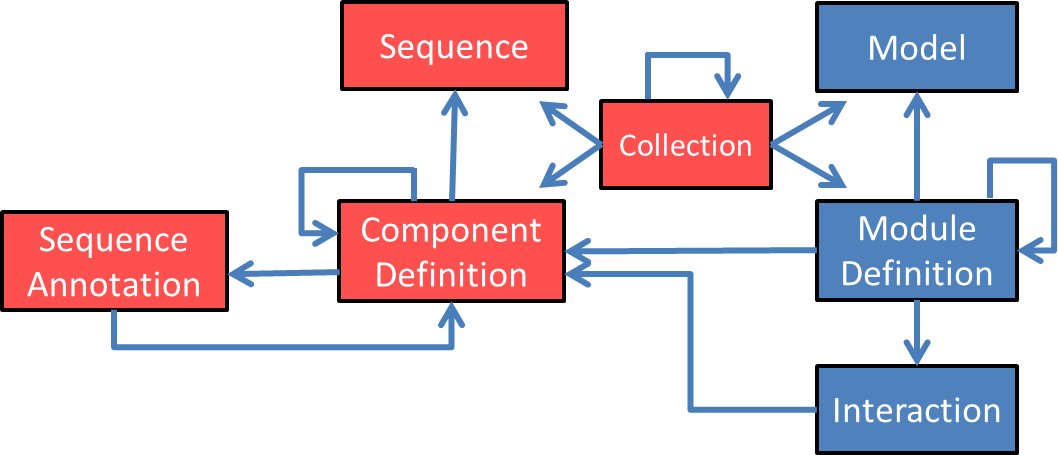
\includegraphics[scale=0.7]{images/OverviewFigforSpec-v7.png}
\caption{Main classes of information represented by the SBOL standard, and their relationships.  Red boxes are classes from the SBOL 1.1 that focused on structure, whereas blue classes are some of the new classes that support the functional aspects of designs.}
\label{images:overview1}
\end{center}
\end{figure}

Whereas Figure~\ref{images:overview1} provides a broad overview of SBOL, Figure~\ref{images:overview2} provides a detailed, implementation-level overview of the class structure for the SBOL 2.0 data model. This figure relies on the semantics of the \emph{Unified Modeling Language} (UML), which will be presented in more detail in the next section. Figure 2 distinguishes between \emph{top level} classes, in green, and other supporting classes (note that Figure 1 also includes all of the top level classes). In Figure 2, dashed arcs represent "refersTo", whereas a solid arrow represents ownership. In UML, the meaning of ownership is that if a parent class is deleted, so are all of its owned children. Thus, a \sbol{Collection} does not own its
\sbol{ComponentDefinition} objects, because these can stand on their own. All of the supporting classes (in orange) must be owned by some top-level class, directly or indirectly. 

% Figure~\ref{images:overview2} provides a more detailed view the the class structure for the SBOL 2.0 data model.  The main, or \emph{top level} classes, are \sbol{Collection}, \sbol{ComponentDefinition}, sbol{Sequence}, \sbol{ModuleDefinition}, and \sbol{Model}.  The key distinction of these classes is that they can stand alone and be referenced by other top level objects (see the dashed arrows between the green boxes).  The purpose of these classes is described above.  Each of these classes is assisted in their purpose by several \emph{child} classes.  The key distinction of a child object is that it is owned by its parent object, and if that parent object is removed, so is the child object.  This ownership is indicated using the solid arrows in the figure.  For example, a \sbol{ComponentDefinition} owns its \sbol{SequenceAnnotation}s.  

\begin{figure}[ht]
\begin{center}
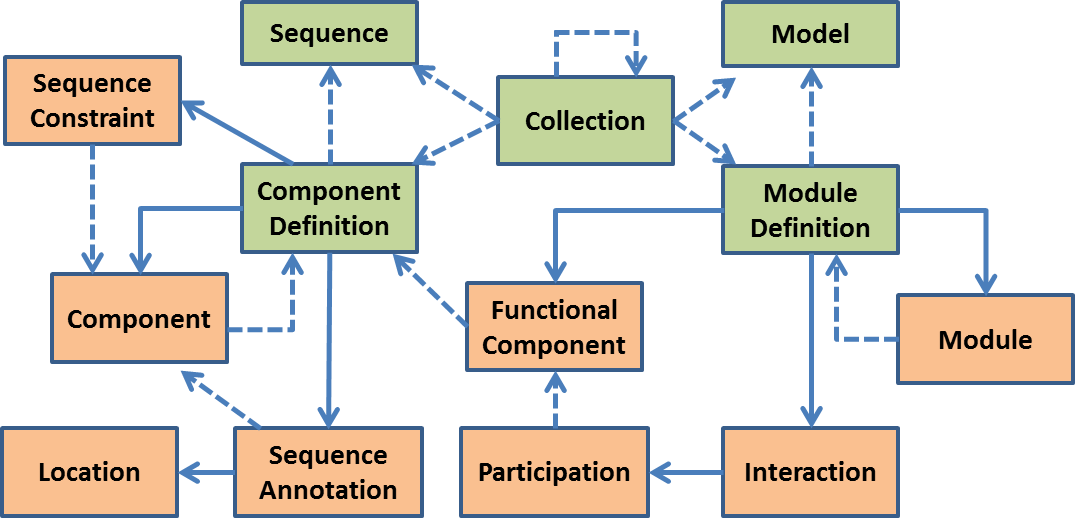
\includegraphics[scale=0.85]{images/OverviewFig2-v4.png}
\caption{Main classes of information represented by the SBOL 2.0 standard, and their relationships.  Green boxes are ``top level'' classes, while the other classes are in support of these classes. Solid arrows indicates ownership, whereas a dashed arrow indicates that one class refers to an object of another class.}
\label{images:overview2}
\end{center}
\end{figure}

Another important difference between the figures is to more appropriately connect the functional side (modules) to the physical side (components). This is accomplished via the class \sbol{FunctionalComponent}. This class allows modules to own their components instances, and yet also allows the physical descriptions (in \sbol{ComponentDefinition}s) to stand on their own. In a similar manner, the ability to have hierarchies of either functional or physical components shown in Figure~\ref{images:overview1} must be broken apart, so that sub-components can be used in multiple functional modules or multiple physical components. Thus, instead of the arc from \sbol{ModuleDefinition} to itself as in Figure~\ref{images:overview1}, our implementation actually divides this notion into two classes, \sbol{ModuleDefinition} and \sbol{Module}. Therefore, a \sbol{ModuleDefinition} does not own the \sbol{ModuleDefinition}s that it uses, but instead it refers to them using the \sbol{Module} objects that it does own.  The identical relationship occurs on the physical side with \sbol{ComponentDefinition} and \sbol{Component}. Finally, SBOL 2.0 provides a few other additional helper classes such as \sbol{Location} that generalizes the positioning information from SBOL 1.1 to allow discontinuous ranges and cuts to be annotated, and \sbol{SequenceConstraint} that generalizes the relative positioning information among \sbol{Component}s.  There is also 
\sbol{Participation}s, which allow \sbol {Interaction} objects to specify the roles of their participants while referencing the \sbol{FunctionalComponent}s, so that these can stand on their own. Finaly, there is the \sbol{MapsTo} class (not shown) that enables connections to be made between \sbol{Component}s and \sbol{FunctionalComponent}s at various levels of the design hierarchy.  The next section provides complete definitions and details for all of these classes.

There is one final critical part of SBOL 2.0, its extension mechanism.  This extension mechanism enables both a framework for application specific information, and a means to prototype representation of data whose format has not yet reached community consensus.  In particular, each SBOL entity can be annotated using the \emph{Resource Description Framework} (RDF). Moreover, application specific entities in the form of RDF documents can be included as \texttt{GenericTopLevel} entities. SBOL libraries makes these annotations and entities available to tools as generic properties and objects that are preserved during subsequent read and write operations. 

% Another important distinction in this diagram are the additional additional \emph{instantiation} classes, \sbol{Component}, \sbol{FunctionalComponent}, and \sbol{Module}.  As described above, a \sbol{ModuleDefinition} may include instantiations of \sbol{ComponentDefinitions}.  These instantiations are called \sbol{FunctionalComponent}s.  Furthermore, \sbol{ModuleDefinition}s and \sbol{ComponentDefinition}s can be constructed hierarchically of instantiations of the same time, and these instantiations are called \sbol{Module}s and \sbol{Component}s, respectively.  Using a software analogy, a \sbol{ComponentDefinition} or \sbol{ModuleDefinition} are a class definition while a \sbol{Component}, \sbol{FunctionalComponent}, or \sbol{Module} are an object of that class type.  

% Finally, one last thing to notice is that child objects can be referenced.  For example, an \sbol{Interaction} is between \sbol{FunctionalComponent} object(s) referenced through the \sbol{Participation} class.  Since this is only a reference, if an \sbol{Interaction} is removed, its \sbol{Participation} objects would be removed but not the \sbol{FunctionalComponent}s that they refer to.  Similarly, \sbol{SequenceAnnotation}s and \sbol{SequenceConstraint}s (provide relative positioning information) only refer to the \sbol{Component}s that they provide positioning information for.


% The \sbol{Sequence} is a fundamental information object for synthetic biology and is needed to reuse components, to replicate synthetic biology work, and to assemble new synthetic biological systems. In designed systems such objects can consist of small chemical molecules, DNAs, RNAs or Proteins. The \sbol{Sequence} object has been designed to encapsulate any of these types of molecules. Small molecule \sbol{Sequence} objects are typically referred to via their chemical formulae. Molecules where sequence specific information is important, such as DNA, RNA and Protein \sbol{Sequence} objects, use the object to incorporate this information. The \sbol{Sequence} object encapsulates this positional information as well as the associated experimental work or other information related to a sequenced molecule.

% \Rtodo{need to make it clear that it includes DNA, RNA, and protein, also smooth the text --JSB made addiitons based upon the suggested changes - KC}

% In the SBOL data model, a structural layer defines the physical arrangement of components in a biological system.  \sbol{ComponentDefinition}s define genetic elements such as promoters, RBSs, CDSs, and terminators, as well as RNA, proteins, and small molecules.  In a structural hierarchy, \sbol{ComponentDefinition}s can contain subcomponents (\sbol{Component}s), which are instances of the \sbol{ComponentDefinition} for that subcomponent.  A functional layer can be defined to describe the behaviors that arise from the structural layer.  \sbol{ModuleDefinition}s contain information about molecular interactions and their participating components.  They can contain \sbol{FunctionalComponent}s that are instances of \sbol{ComponentDefinition}s that can be assigned functional properties, and they can also contain other modules in a functional hierarchy.  The functions and interactions of these components and other modules within the \sbol{ModuleDefinition} can be quantitatively or qualitatively described using a \sbol{Model}. The \sbol{SequenceAnnotation} object defines data associated the \sbol{Sequence} and \sbol{ComponentDefinition} objects that is needed beyond basic definitions. This can refer to local annotations of the object as well as a container for URIs to external information sources. 


% SBOL includes different entities to describe such genetic circuits. Genetic elements such as a promoter, ribosome binding site (RBS), coding sequence (CDS), or terminator are defined with the \sbol{ComponentDefinition} entity. Their instances are reused in different designs via the \sbol{Component}s that refer to corresponding \sbol{ComponentDefinition}s. \sbol{ComponentDefinition}s can also represent proteins, RNAs or small molecules. They are associated with sequence information such as nucleotides aminoacids or chemical structure. A full description of a genetic circuit is then represented using  \sbol{ModuleDefinition}s which contains information about molecular interactions and their participating components. Modules can be associated with quantitative or qualitative models using the \sbol{Model} entity, which is used to point to the actual location of a model. 
% \sbol{SequenceAnnotation}s can be used to carry data associated with the successful running of that model on another computer, can be used to point towards sources of some or all of the circuit and the location of experimental data associated with the development of the model.

% \Rtodo{Need to also explain annotation --JSB
% Provided some text for review describing annotation - KC}



% SBOL facilitates the design of complex systems using hierarchical composition. In addition to using simple genetic elements in a modular fashion, modules that are composed of multiple, different components can also be reused. Such modules can expose some of the design components as inputs and outputs, which can be connected to components from other modules using \sbol{MapsTo} entities.


% \Ctodo{This needs to be clarified.  Do we really want to explain MapsTo here? -JSB}
% \Ctodo{it's not in the diagram. So it should be removed or dealt with in the figure and earlier in the text- KC}

% \Ctodo{Explain why it is important to separate definitions from instantiations?}

% \LDtodo{The motivation for separating structural and functional considerations is not explained.  Which class names are structural, which class names are functional, and how are the two connected?  Do all structural components require a functional counterpart?  If not, explain why only a subset of structural components would have functional definitions.}

% \Ctodo{As a person reading about SBOL2 for the first time, I rank this as the most important section.  While the document should be technically focused overall, this section is your chance to concisely tell someone who won't read the whole document about the take-home messages for the new data model.}

% \LDtodo{Why are URI's needed for Components?  Why not just for ComponentDefinitions?  Is there anything in SBOL that does not require a URI?}
% \Ctodo{Also briefly mention URI}

% \Ctodo{Make sure we explain about annotations up in the motivation and overview, since it's really, really important.}

% The same toggle switch is now displayed using two LacI and TetR inverter submodules in figure \ref{images:toggleswitch_modular}. The LacI inverter uses LacI as input and produces the TetR output, and the TetR inverter uses TetR as input and produces the LacI output. These inputs and outputs are mapped in a parent module.

% Removed as redundant:
%-----------------------------------------------------------------------------
%\section{Introduction}
% -----------------------------------------------------------------------------
%While the first version of the Synthetic Biology Open Language (SBOL) has been adopted by several academic and commercial genetic design automation (GDA) software tools, it only covers a limited range of the requirements for a standardized exchange format for synthetic biology. The SBOL 2.0 specification revises version 1.1, enabling the representation of a wider range of components with and without sequences, including RNA components, protein components, small molecules, and molecular complexes. Additionally, the latest SBOL can be used to convey the intended function of a design, as well as its structural composition. 
%This dichotomous representation of the structural and functional features of a design is a paradigm applied to great success in electrical and computer engineering, and is essential for the development of design automation software in synthetic biology.
%
%The goal of this specification is to define the terminology and relationships used to describe biological designs. In order to provide a shared understanding between engineers seeking to exchange biological designs, SBOL provides a common definition of the concepts needed. As much as possible, we attempt to make explicit the meaning of all terminology and data structures.


% % -----------------------------------------------------------------------------
% \section{Overview of SBOL}
% % -----------------------------------------------------------------------------
% Typically, information about a  genetic circuit includes the order of its constituents and their descriptions. The exact locations of these constituents and their sequences allow genetic circuits to be defined unambiguously, and reused in other designs. Interactions between these constituents are then used to construct biologically plausible designs. 

% In the figure below, a simple toggle switch system is displayed, in which LacI and TetR repress each other's genes transcriptionally. The toggling of the system  is controlled by adding IPTG to deactivate LacI, and ATC to deactivate TetR. The components of the system includes genetic elements, proteins, small molecules.

% \begin{figure}[ht]
% \begin{center}
% 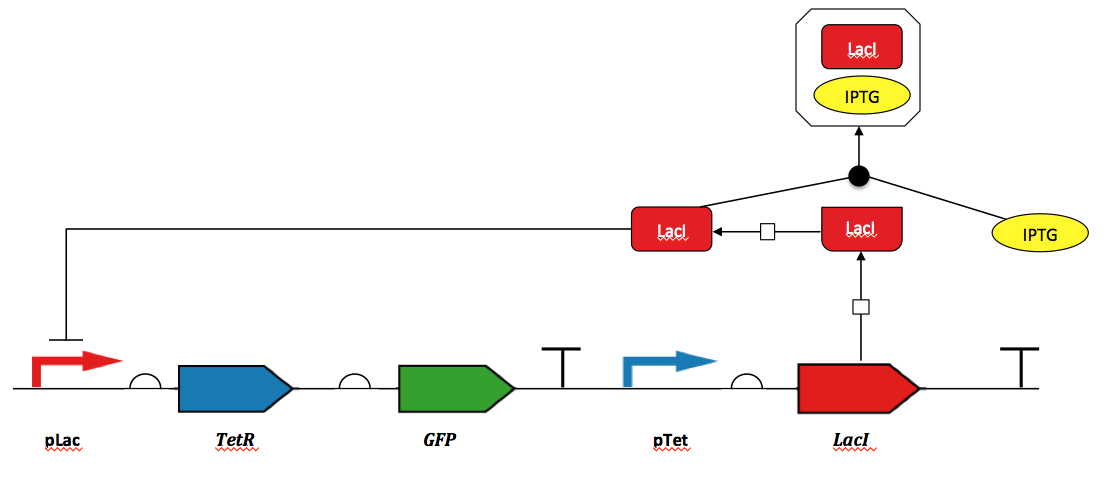
\includegraphics[scale=0.4]{images/toggleswitch_flat}
% \caption[]{An example toggle swicth genetic circuit. }
% \label{images:toggleswitch_flat}
% \end{center}
% \end{figure}

% SBOL includes different entities to describe such genetic circuits. Genetic elements such as promoters, RBS, CDSs and terminators are defined with the \sbol{ComponentDefinition} entity. Their instances are reused in different designs via the \sbol{Component}s that refer to corresponding \sbol{ComponentDefinition}s. \sbol{ComponentDefinition}s can also represent proteins, RNAs or small molecules. They are associated with sequence information such as nucleotides aminoacids or chemical structure. A full description of a genetic circuit is then represented using  \sbol{ModuleDefinition}s which contains information about molecular interactions and their participating components. Modules can be associated with quantitative or qualitative models using the \sbol{Model} entity, which is used to point to the actual location of a model.


% SBOL facilitates the design of complex systems using hierarchical composition. In addition to using simple genetic elements in a modular fashion, modules that are composed of multiple, different components can also be reused. Such modules can expose some of the design components as inputs and outputs, which can be connected to components from other modules using \sbol{MapsTo} entities.